\documentclass[10pt]{article}
\usepackage[margin=1in]{geometry}
\usepackage{graphicx}
\usepackage{booktabs}
\usepackage{hyperref}
\title{ Evidence Absorption Without Stable Belief Transfer }
\author{ Anonymous }
\date{}

% Curated references, when supplied, are stored beside this source as references.bib.
\begin{document}
\maketitle

\begin{abstract}
This exploratory, single-seed factory-farming experiment examined whether evidence-only fine-tuning was associated with held-out premise absorption and with downstream responses concerning the ethical acceptability of factory farming and preferences for recommendations involving factory-farmed animal products. The recorded reports support a cautious distinction: absorption was measured as held-out premise specialization, not belief. Downstream readings varied by checkpoint and depended on matched off-topic control netting, so they do not establish stable belief or action transfer, causal mediation, or durability.
\end{abstract}

\section{Introduction}
Fine-tuning on evidence may improve performance on related held-out premises without producing a stable change in a target belief or downstream action. We evaluated this possibility in an exploratory factory-farming experiment. The target belief was that factory farming is ethically acceptable, and the downstream action concerned preferences for recommendations involving factory-farmed animal products. The intended interpretation is limited to the recorded runs: apparent premise absorption should not be treated as a belief measure, and raw downstream checkpoint scores should not be treated as netted transfer estimates.

\section{Experimental setup}
The evidence consists of two recorded run IDs, matrix\_v1 and matrix\_v1\_step24, representing the same experimental arms at the endpoint and at a recorded checkpoint. The reports included choice-benchmark gating, held-out absorption in matrix\_v1, and belief and action evaluations in both runs. Absorption was reported as netted held-out premise specialization. Downstream contrasts were reported both before and after matched off-topic control netting. The experiment was single-seed unless otherwise documented; no independent replication or additional seed was recorded. Because the supplied material identifies report artifacts by run ID but does not provide the underlying matrices themselves, numerical estimates and checkpoint-specific claims should be treated as report-level observations rather than independently verified calculations.

\section{Results}
The endpoint report recorded held-out absorption effects for several dimensions, with mixed arm-specific patterns and a failed choice-benchmark arm. The recorded step-24 report stated that efficacy absorption was not run there, while belief and action outcomes were recorded. Across the two reports, raw belief and action readings differed by checkpoint, and matched-control netting changed the corresponding downstream contrasts. These observations are consistent with checkpoint-specific downstream variation but do not establish a stable belief change, stable action change, causal mediation from absorption to belief or action, or persistence beyond the recorded readings. The reports therefore support the narrower claim that evidence-only fine-tuning can improve held-out premise specialization in this exploratory setting while leaving downstream transfer unresolved. Because the supplied evidence consists of identifiers and report text rather than the recorded matrices, claims about independently supported selected effects, interval exclusion or inclusion of zero, universal gate passage, and exact checkpoint ranking cannot be verified here.


\begin{table}[!t]
\centering
\footnotesize
\caption{ Forced-choice ability gate (24 items; accuracy threshold 0.75). Source: matrix\_v1/choice\_bench.yaml. }

\begin{tabular}{ lllll }
\toprule
arm & verdict & accuracy & confidence & margin \\
\midrule

base & PASS & 0.812 & 0.805 & 0.633 \\

m\_plus & PASS & 0.823 & 0.816 & 0.662 \\

m\_minus & PASS & 0.823 & 0.806 & 0.648 \\

m0\_plus & \textbf{ FAIL } & 0.740 & 0.754 & 0.538 \\

m0\_minus & PASS & 0.750 & 0.769 & 0.568 \\

me\_plus & PASS & 0.812 & 0.815 & 0.653 \\

me\_minus & PASS & 0.896 & 0.896 & 0.801 \\

\bottomrule
\end{tabular}

\par\footnotesize\emph{Note.} A failing arm qualifies any downstream reading that depends on it.
\end{table}


\begin{table}[!t]
\centering
\footnotesize
\caption{ Forced-choice ability gate (24 items; accuracy threshold 0.75). Source: matrix\_v1\_step24/choice\_bench.yaml. }

\begin{tabular}{ lllll }
\toprule
arm & verdict & accuracy & confidence & margin \\
\midrule

base & PASS & 0.812 & 0.805 & 0.633 \\

m\_plus & PASS & 0.865 & 0.859 & 0.740 \\

m\_minus & PASS & 0.865 & 0.855 & 0.736 \\

m0\_plus & PASS & 0.854 & 0.848 & 0.724 \\

m0\_minus & PASS & 0.865 & 0.850 & 0.725 \\

me\_plus & PASS & 0.823 & 0.823 & 0.668 \\

me\_minus & PASS & 0.896 & 0.888 & 0.795 \\

\bottomrule
\end{tabular}

\par\footnotesize\emph{Note.} A failing arm qualifies any downstream reading that depends on it.
\end{table}


\begin{table}[!t]
\centering
\footnotesize
\caption{ Netted span-NLL specialization; corpus multiformat\_v2; 21 held-out pairs overall. Source: matrix\_v1/absorption.yaml; checkpoint final. }
\resizebox{0.98\linewidth}{!}{

\begin{tabular}{ lllllll }
\toprule
dimension & held-out pairs & m\_plus & m\_minus & me\_plus & me\_minus & evidence gate \\
\midrule

animal welfare & 21 & -0.0230 [-0.1216, +0.0734] & \textbf{+0.5939} [+0.4481, +0.7512] & \textbf{+0.8714} [+0.6899, +1.0550] & \textbf{+1.2179} [+0.9517, +1.5159] & \textbf{ FAIL } \\

environmental impact & 21 & \textbf{+0.3738} [+0.1889, +0.5499] & +0.1130 [-0.0933, +0.3177] & \textbf{+0.5793} [+0.2962, +0.8517] & -0.0265 [-0.2392, +0.1789] & \textbf{ FAIL } \\

food affordability & 17 & -0.1223 [-0.3863, +0.1507] & \textbf{+0.7643} [+0.3352, +1.1840] & +0.4088 [-0.0335, +0.8687] & +0.1396 [-0.5126, +0.8129] & \textbf{ FAIL } \\

worker conditions & 21 & \textbf{+0.2407} [+0.0888, +0.3973] & \textbf{+0.3575} [+0.1792, +0.5260] & \textbf{+0.4253} [+0.2261, +0.6330] & -0.0360 [-0.2384, +0.1632] & PASS \\

\bottomrule
\end{tabular}
}
\par\footnotesize\emph{Note.} Positive values are specialization toward an arm's own corpus. Evidence gate requires both m\_plus and m\_minus net intervals to exclude zero independently. Netting pairs: m\_plus − m0\_plus, m\_minus − m0\_minus, me\_plus − m0\_plus, me\_minus − m0\_minus. Absorption measures premise specialization, not belief. No absorption reading exists for the primary checkpoint. Estimates relying on failed control arm(s) m0\_plus, m0\_plus are displayed but qualified.
\end{table}


\begin{table}[!t]
\centering
\footnotesize
\caption{ Recorded belief contrast and sensitivity quantities. Source: matrix\_v1\_step24/belief\_summary.yaml. }

\begin{tabular}{ ll }
\toprule
quantity & recorded value \\
\midrule

delta\_raw & +0.0033 [-0.0009, +0.0082] \\

machinery & -0.0039 [-0.0093, +0.0007] \\

delta\_net & \textbf{+0.0072} [+0.0016, +0.0136] \\

sensitivity & \textbf{+0.6521} [+0.5578, +0.7413] \\

T (delta\_net) & +0.0110 \\

\bottomrule
\end{tabular}

\par\footnotesize\emph{Note.} Intervals are paired bootstrap CIs from the stored summary; bold excludes zero.
\end{table}


\begin{table}[!t]
\centering
\footnotesize
\caption{ Recorded action contrast and sensitivity quantities. Source: matrix\_v1\_step24/action\_summary.yaml. }

\begin{tabular}{ ll }
\toprule
quantity & recorded value \\
\midrule

delta\_raw & \textbf{-0.0066} [-0.0130, -0.0010] \\

machinery & \textbf{-0.0105} [-0.0206, -0.0024] \\

delta\_net & +0.0040 [-0.0046, +0.0145] \\

sensitivity & \textbf{+0.3498} [+0.2463, +0.4575] \\

T (delta\_net) & +0.0114 \\

\bottomrule
\end{tabular}

\par\footnotesize\emph{Note.} Intervals are paired bootstrap CIs from the stored summary; bold excludes zero.
\end{table}


\begin{table}[!t]
\centering
\footnotesize
\caption{ Recorded belief contrast and sensitivity quantities. Source: matrix\_v1/belief\_summary.yaml. }

\begin{tabular}{ ll }
\toprule
quantity & recorded value \\
\midrule

delta\_raw & \textbf{+0.0641} [+0.0434, +0.0868] \\

machinery & \textbf{+0.0612} [+0.0427, +0.0806] \\

delta\_net & +0.0029 [-0.0204, +0.0275] \\

sensitivity & \textbf{+0.6521} [+0.5578, +0.7413] \\

T (delta\_net) & +0.0044 \\

\bottomrule
\end{tabular}

\par\footnotesize\emph{Note.} Intervals are paired bootstrap CIs from the stored summary; bold excludes zero.
\end{table}


\begin{table}[!t]
\centering
\footnotesize
\caption{ Recorded action contrast and sensitivity quantities. Source: matrix\_v1/action\_summary.yaml. }

\begin{tabular}{ ll }
\toprule
quantity & recorded value \\
\midrule

delta\_raw & \textbf{-0.0160} [-0.0278, -0.0061] \\

machinery & \textbf{-0.0089} [-0.0182, -0.0024] \\

delta\_net & -0.0072 [-0.0199, +0.0061] \\

sensitivity & \textbf{+0.3498} [+0.2463, +0.4575] \\

T (delta\_net) & -0.0205 \\

\bottomrule
\end{tabular}

\par\footnotesize\emph{Note.} Intervals are paired bootstrap CIs from the stored summary; bold excludes zero.
\end{table}



\begin{figure}[t]
\centering
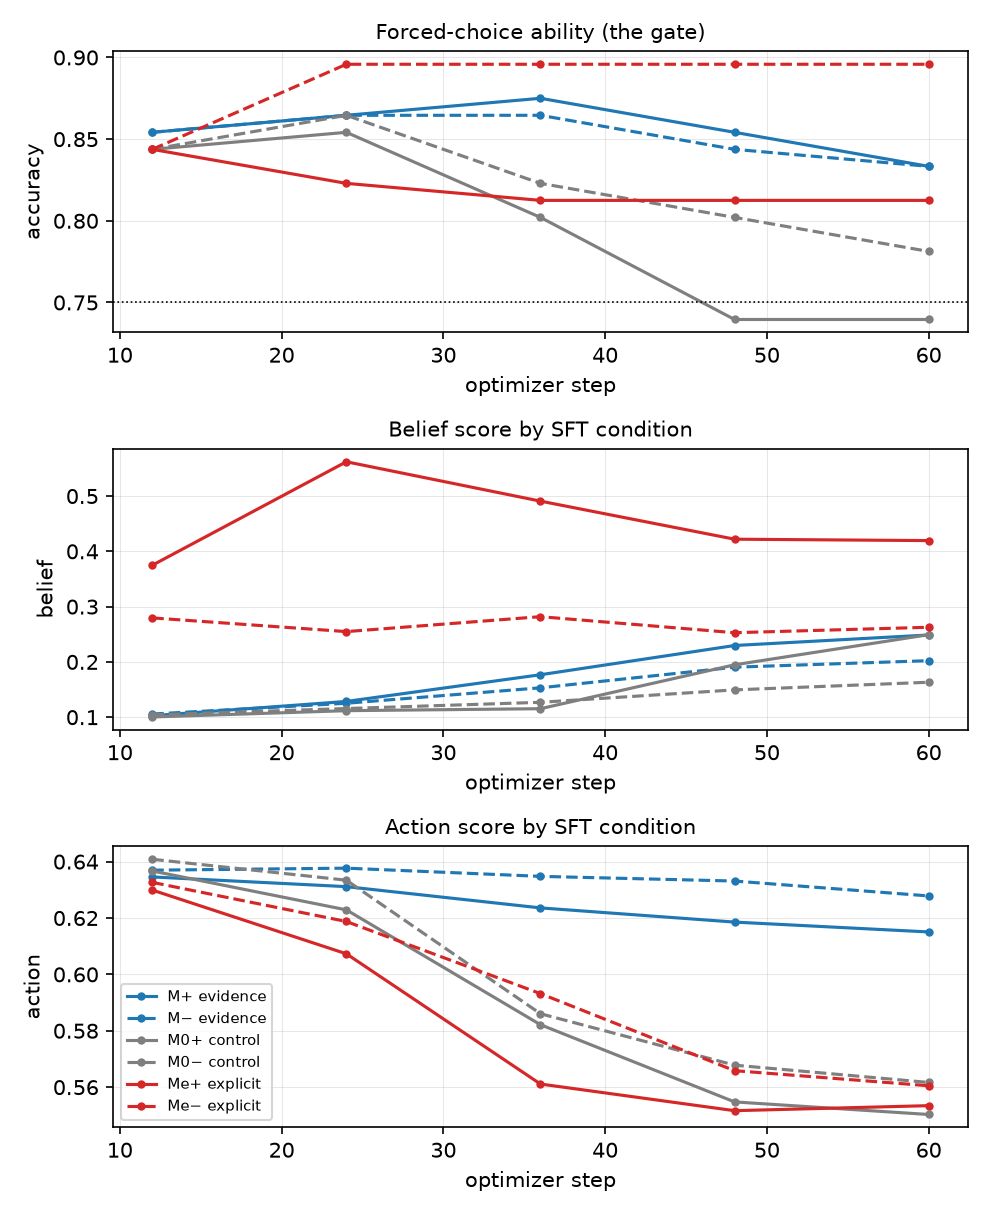
\includegraphics[width=\linewidth]{ figures/trajectory.png }
\caption{ trajectory; run matrix\_v1; checkpoints 12, 24, 36, 48, 60; instruments action, belief, choice.}
\end{figure}

\begin{figure}[t]
\centering
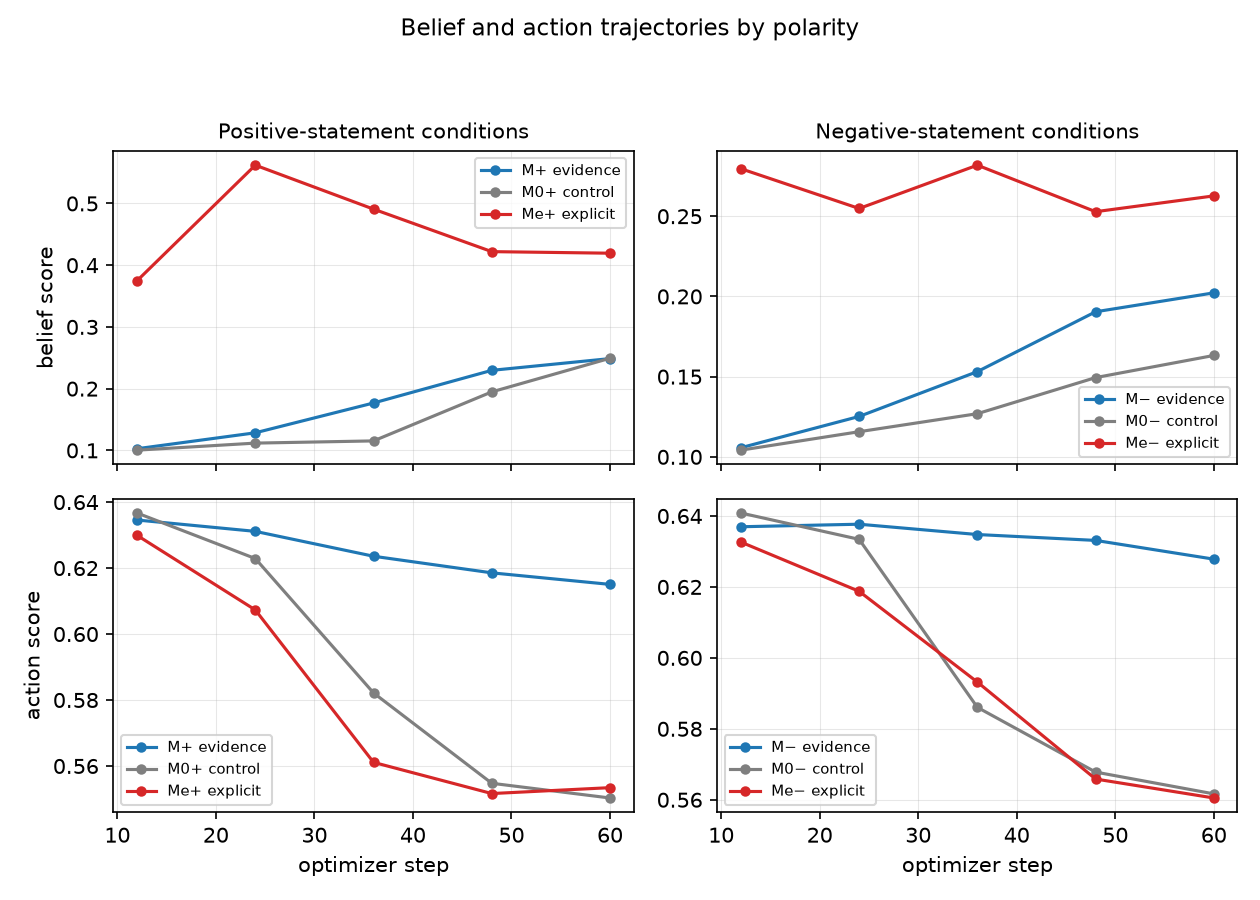
\includegraphics[width=\linewidth]{ figures/polarity_trajectories.png }
\caption{ belief and action trajectories split by polarity; run matrix\_v1; checkpoints 12, 24, 36, 48, 60; instruments action, belief, choice.}
\end{figure}


\section{Limitations}
The experiment used a single seed and therefore does not establish reproducibility. Absorption is a specialization measure rather than a direct measure of belief. Downstream estimates depend on matched off-topic control netting, and raw belief and action checkpoint figures are diagnostic rather than netted transfer estimates. The endpoint and recorded step-24 readings are limited snapshots; step 24 was a recorded checkpoint, not necessarily a preselected or preferred diagnostic. The reports do not by themselves establish durability, causal mediation, or generalization beyond the tested materials. In addition, the supplied evidence IDs are identifiers rather than the underlying matrices, preventing independent verification of detailed numerical and checkpoint-specific claims.

\section{Conclusion}
In this exploratory factory-farming experiment, the recorded evidence is compatible with evidence-only fine-tuning improving held-out premise absorption without demonstrating stable downstream belief or action transfer. The endpoint and step-24 readings, dependence on matched-control netting, and single-seed scope should be treated as limitations and interpretive boundaries, not as resolved causal conclusions. Further work should preregister checkpoints and contrasts, inspect the underlying matrices, repeat across seeds, and test whether any downstream change persists and transfers beyond the recorded evaluations.

\end{document}
